\section{Introduction}
\label{sec:intro}

Consider a data warehouse scenario: a database describes how a set of
\emph{measures} varies along several \emph{dimensions}. To work with this
database, analysts need a lot of prior knowledge: which dimensions and measures
they are interested in, where interesting patterns are hidden in the cube,
which dependencies among dimensions and measures exist, and much more.  Manual
exploration may expose some of this knowledge, but the success of this method
depends entirely on chance and intuition. In contrast to this, we aim at a
semi-automated exploration.  We want to assist the humans in understanding how
measures are distributed, where unexpected measures appear, and where
interesting dependencies between dimensions and measures arise.

We believe that automating query generation is essential to make analysts
more productive. Informations which are trivial for domain experts are not
necessarily so for data specialists. Besides, experts themselves may need
guidance. Consider for instance Figure \ref{intro}. The table shows a small
extract from a dataset of astronomical observations\footnote{This dataset come
from the LOFAR research programme, 21 May 2012, the Netherlands}. We want
to observe the \emph{brightness} of more than 100,000 sources, taken at
different times, frequency ranges and with different precisions. In total,
there are more than fifty dimensions. Even for an astronomer, this dataset
cannot be understood by intuition alone. We need intelligent tools to provide
guidance.  The bottom picture illustrates what we expect from our query
generation system: a simpler low dimension view of dependent dimensions and
measures, which reveals particularly bright or large sources. Thanks to this
view, anyone can quickly perceive interesting regions in the database.

\begin{figure}[t!]
\centering
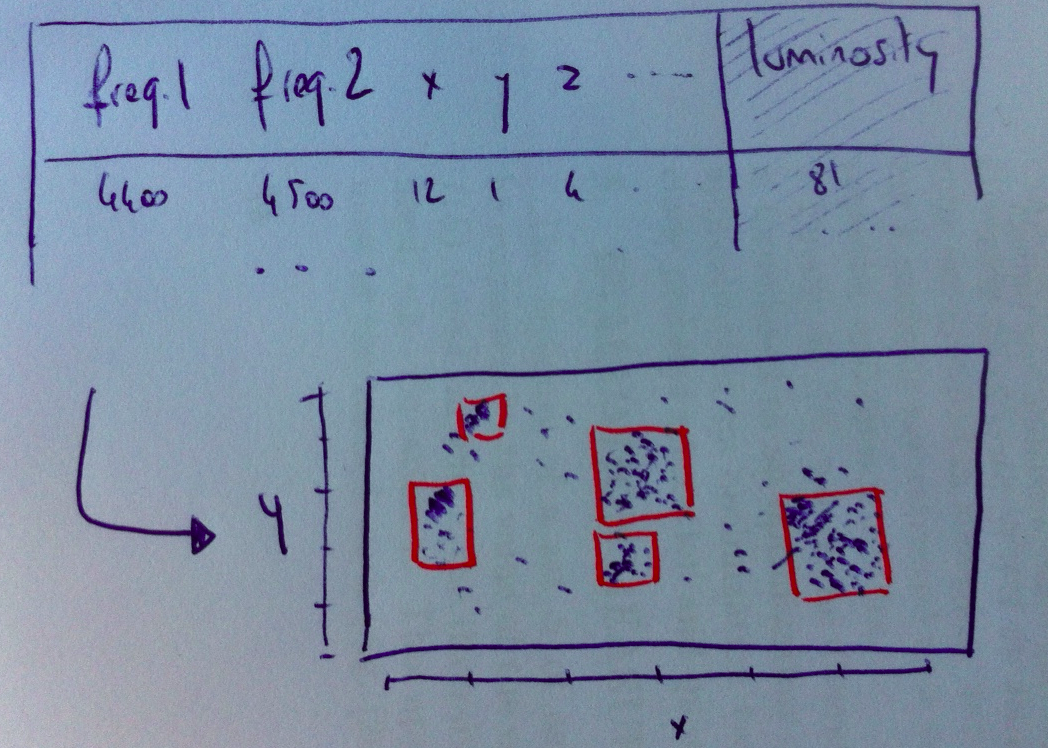
\includegraphics[width=0.8\columnwidth]{images/intro}
\caption{Revealing interesting regions}
\label{intro}
\end{figure}

Semi-automated exploration of data cubes is fundamentally challenging for two
reasons. The first reason is obvious: how do we recognize ``interesting''
queries?  The diversity of opinions in the literature is rather depressing.
What is interesting for a user can be extremely boring for another. The second
problem is practical.  Suppose that we had a universal measure of interest, how
could we explore the search space fast enough to find the interesting queries?

Many authors have proposed semi-automated (or discovery-driven) exploration
frameworks in the past. Typically, they introduce a fixed ``interestingness''
model, then the exploit the particularities of their model to speed up
computations.  For instance, a seminal work was presented by Sarawagi et al.
\cite{sarawagi1998discovery}. According to their paper, the most interesting
queries are the most ``surprising'' ones.  They suggest to build a (log-linear)
model over the data, and identify the largest deviations. More recently, Dash
et al.\cite{dash2008dynamic} proposed a facet selection method, also based on
surprise. Nevertheless, given the diversity of users and requirements, are
these interestingness models \emph{really} interesting?

In this paper, we introduce \textit{Claude}, a \emph{generic} query generation
system.  The idea is to delegate the choice of interestingness, and
focus on the exploration. \emph{Claude lets users describe what they are
looking for.  Given this input, it explores the database and reveals
interesting OLAP views}. 

Claude's users assign a value to each tuple in the database. We call this value
the \emph{target}. It can come from the raw data (e.g., the brightness of light
sources), a calculation (e.g., a ``surprise'' score from the litterature), or
manual effort. Claude's job is to present the ``big picture'': it explains how
the target is distributed across the database, and what influences it. To do
so, it operates in two steps. First, it explores the database for interesting
projections. Then, for each projection, it reveals areas with unusual target
values.  Performance is a major
challenge. We introduce two algorithms.  The first one is exact and based on a
systematic level-wise search paradigm.  The second one is a much faster and
based on a relaxation of our model and a heuristic search.
